\section{Design}

\subsection{Data Collection}

The over arching algorithm for collecting data is shown in Figure \ref{fig:main-flow}. For each bus route the following steps occur. \\

\begin{figure}[H]
\begin{center}
    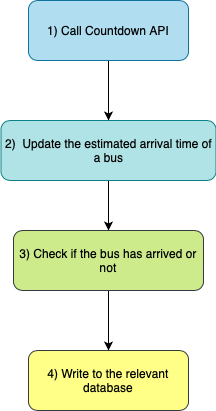
\includegraphics[keepaspectratio, width=6cm]{Images/Data-Collection-new-overarch.png}
    \caption{Overarching data collection algorithm}
    \label{fig:main-flow}
\end{center}
\end{figure}

\textbf{1) Call Countdown API:} Data provided by the Countdown API is stop centric. This means that stop information is crucial to the requests made. Therefore, before the Countdown API can be called, the Stoppoints API must be called to determine the stop ids of all of the stops on a bus route. \\ 

Stoppoints could be called before each Countdown call, however, this is a waste of time since as mentioned in Section \ref{section:tfl-api} Stoppoints returns a mix of valid and invalid stop ids. Time would have to be spent filtering the Countdown responses to see which have returned expected arrival times and which have returned HTTP errors. Furthermore, it is much faster to access a list of valid stop ids from a database than to retrieve information from an API call. \\

Therefore, it is more computationally efficient to call the Stoppoints API for each bus route used in the data collection process once a week and store the response in a database. Since Countdown only requires the unique national identifier (\texttt{naptanID}) of the bus stop, it is only necessary to extract this parameter from the API response for each stop. The common English name of the stop (\texttt{commonName}) is also extracted from the API for ease of data analytics later on. The  \texttt{valid\_stop\_ids\_route} table stores the list of valid stop ids and its respective plain English name for that particular route. A snippet of valid stops for bus route 9 is shown in Figure \ref{fig:valid-stops-db}. The database design is shown in Figure \ref{fig:valid-stops-db-design}. \\

\begin{figure}[H]
\centering
\begin{minipage}{.65\textwidth}
  \centering
  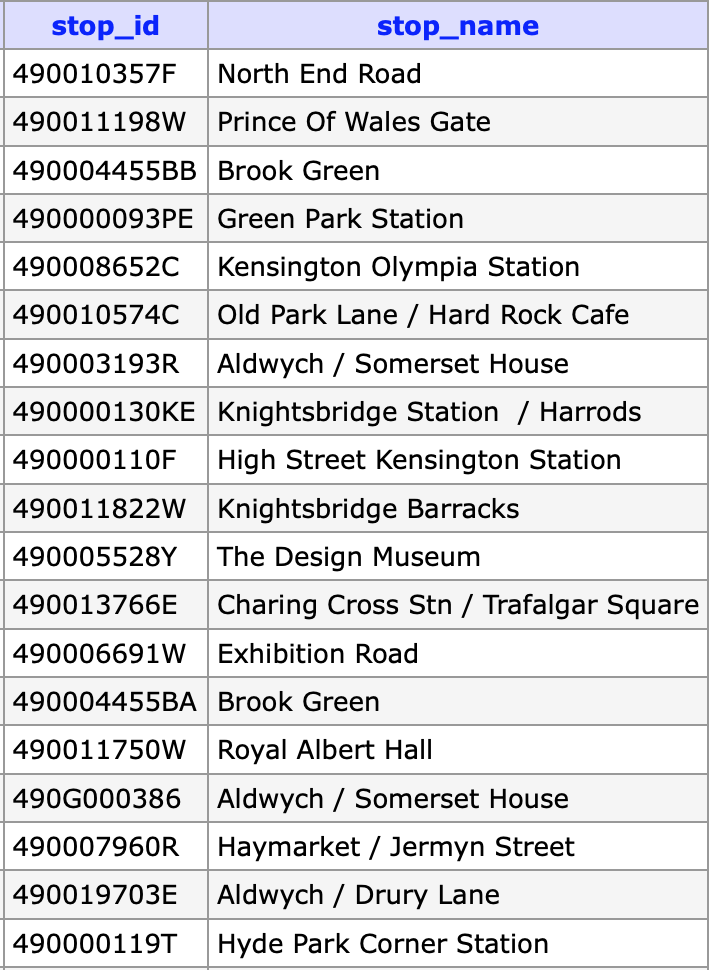
\includegraphics[width=.6\linewidth]{Images/valid-stops.png}
  \caption{Valid Stop Ids Example}
  \label{fig:valid-stops-db}
\end{minipage}%
\begin{minipage}{.35\textwidth}
  \centering
  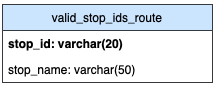
\includegraphics[width=.8\linewidth]{Images/database-diagram-validstops.png}
  \caption{Valid Stop Ids Table}
  \label{fig:valid-stops-db-design}
\end{minipage}
\end{figure}

\textbf{2) Update the estimated arrival time of a bus: } Countdown is called continuously every 30 seconds because as mentioned in Section \ref{section:tfl-api} the information is only updated at source every 30 seconds. If the new expected arrival time returned from the API call is the same as what the database already holds, there is no need to update the item. Otherwise, the database updates both the bus' expected arrival time and the time of the API request. \\

Figure \ref{fig:more-accurate-closer-to-eta} shows two different expected arrival times for Dalgarno Gardens on bus route 7. The figure demonstrates how the predicted arrival time for the same vehicle changes the closer it gets to the actual arrival time. Therefore, data much be collected and updated continuously in order to get as accurate an inferred arrival time as possible.

\begin{figure}[H]
\begin{center}
    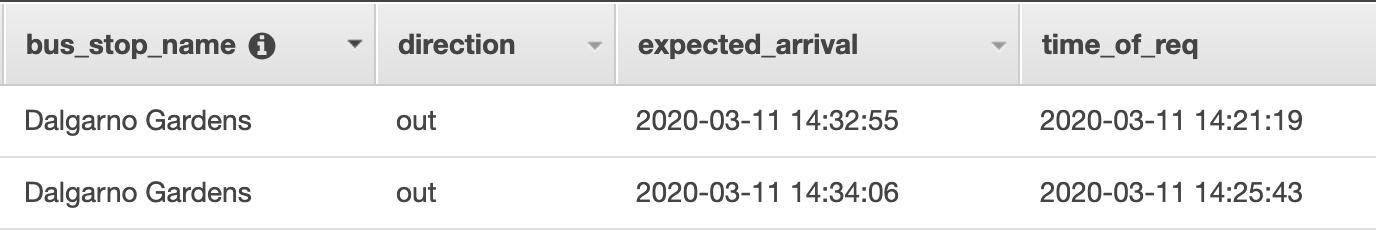
\includegraphics[keepaspectratio, width=15cm]{Images/updated-arrival-time-as-request-is-closer-to-real-time.png}
    \caption{Route 7 data for a particular vehicle X}
    \label{fig:more-accurate-closer-to-eta}
\end{center}
\end{figure}

\textbf{3) Check if the bus has arrived or not:} Figure \ref{fig:check-if-bus-arrived} shows the flow of logic which takes place in order to ascertain whether a bus has arrived or not. If a bus \textit{A} is due to arrive at time \textit{X}, when Countdown is called at time \textit{X} and \textit{A} does not appear in the response, it cannot be assumed that \textit{A} has arrived at time \textit{X}. It is possible that there could have been a glitch in the system and \textit{A} has just temporarily vanished. Therefore, the algorithm waits 5 minutes after time \textit{X} and if \textit{A} does not appear in the Countdown response again, then it can be inferred that \textit{A} did indeed arrive at time \textit{X}. However, if during the 5 minutes after time \textit{X} bus \textit{A} reappears, this implies that \textit{A} will return with a new expected time \textit{Y} and thus did not arrive at time \textit{X}. 

\begin{figure}[H]
\begin{center}
    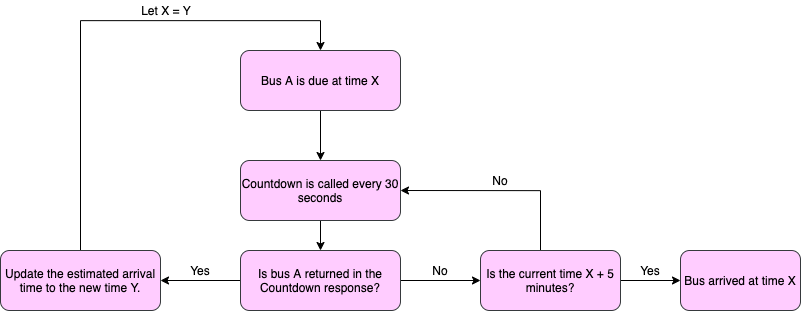
\includegraphics[keepaspectratio, width=16cm]{Images/datacollection-flow.png}
    \caption{Check if the bus has arrived or not}
    \label{fig:check-if-bus-arrived}
\end{center}
\end{figure}

\textbf{4) Write to the relevant database:} Figure \ref{fig:databases} shows the designs of each of the databases described below.

\begin{itemize}
    \item \texttt{bus\_information\_route} stores information on buses that haven't arrived yet for a particular route.
    \item \texttt{bus\_arrivals\_route} stores information on all buses that have arrived for this route. 
\end{itemize}

\begin{figure}[H]
\begin{center}
    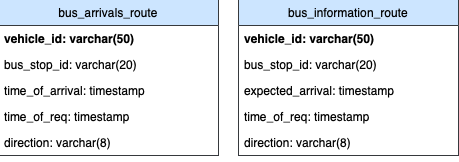
\includegraphics[keepaspectratio, width=12cm]{Images/database-diagrams.png}
    \caption{Databases}
    \label{fig:databases}
\end{center}
\end{figure}

Recall the example Countdown responses in Section \ref{section:tfl-api} for buses arriving at North End Road on bus route 9. Figure \ref{fig:arrived-database} shows how the JSON information has been converted into strings and datetime objects. Specifically, bus \textit{14510} was predicted to arrive at \textit{1589526117000} in UNIX epoch time. This converts to \textit{07:01:57} as seen in the third row of Figure \ref{fig:arrived-database}. The vehicle\_id is a combination of the actual bus id, the stop id, the date of arrival, the direction and the journey number that the bus is on. This is necessary because a particular bus e.g. bus with id \textit{14510} will complete more than one full journey on its route. \\

\begin{figure}[H]
\begin{center}
    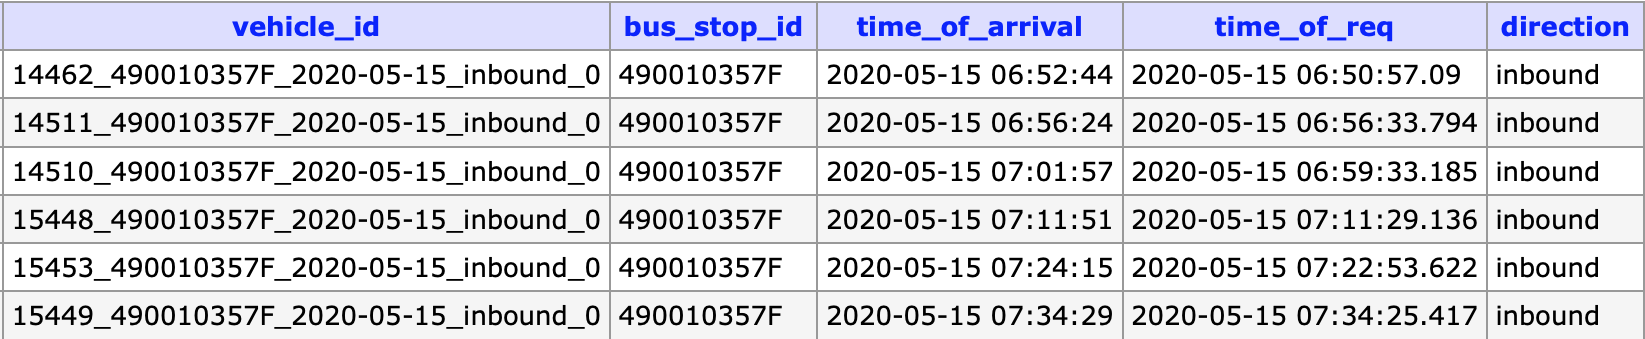
\includegraphics[keepaspectratio, width=16cm]{Images/arrived-northendroad.png}
    \caption{Buses that arrived at North End Road}
    \label{fig:arrived-database}
\end{center}
\end{figure}

\subsubsection{Technology Choices}

This project is quite broad in terms of implementation decisions, therefore, there was no necessity to pick any particular language. Since I had done a lot of projects in Python in my final year of university and because Python has a lot of support online, I chose to write the code that performs the API calls and logic for whether a bus has arrived in Python. \\

Initially, the data collection code was hosted on Amazon Web Services (AWS), using AWS Lambdas to run the data collection functionality and AWS DynamoDB to store the data. AWS Lambda allows code to be run without requiring a server to be provisioned or managed. AWS DynamoDB is a key-value NOSQL database. I chose AWS because its free tier had generous usage and its services worked cohesively together easily and smoothly. Unfortunately, approximately two months into the data collection stage - the code having been left running while I moved on to other parts of the project - I realised that I had exceeded the free tier usage. Therefore, I had to relocate my code onto the DoC Cloud VM. This was chosen because there is less of a memory/usage capacity limit and furthermore is free. \\

The data collection code has now been put in a Docker container. This is because it made it much easier to move the code between environments as it already held all the dependencies needed to run the code. \\

The current data collection code has now changed to use a PostgreSQL database, which is a relational database. This change was done partly because by this point I had already begun writing the code to do the arrival time predictions and I found that it was much more convenient to query for values instead of having to loop through the key value pairs. 

\subsection{Data Exploration}
\label{section:data-exploration}

It is important to explore the dataset collected before building the models in order to understand it better. This could be by discovering patterns, spotting outliers or understanding relationships between variables. \\

For each of the bus routes, graphs were plotted to show the total number of buses arriving at bus stops at different times of day. This helped to see the pattern of numbers of buses according to time of day. It was hypothesised that there would be more buses running during the day than during the night. This was supported by the graphs, for example, from Figure \ref{fig:spread-of-buses-over-day-6} it can be seen that for route 6 during the day, approximately between 0700-1700, there are many more buses on the road, compared to say 2100-0300. 

\begin{figure}[H]
\begin{center}
    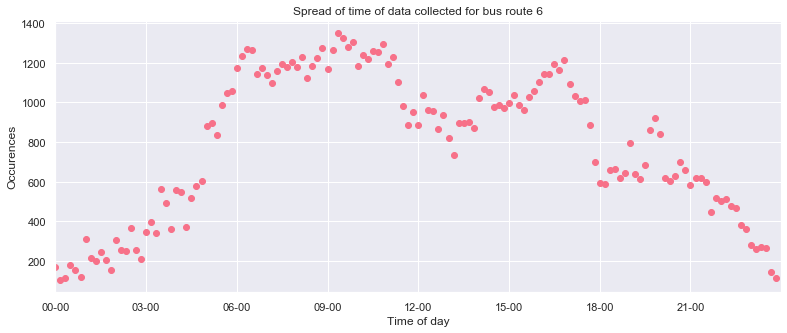
\includegraphics[keepaspectratio, width=15cm]{Images/exploration-spreadofbus6.png}
    \caption{Number of buses during the day for route 6}
    \label{fig:spread-of-buses-over-day-6}
\end{center}
\end{figure}

Graphs were also plotted to see the total number of buses arriving at bus stops on different days of the week. It was hypothesised that there would be more buses running during weekdays compared to the weekend. However, it can be seen from Figure \ref{fig:spread-of-buses-over-week-6} that there did not seem to be a pattern indicating that the hypothesis was correct.

\begin{figure}[H]
\begin{center}
    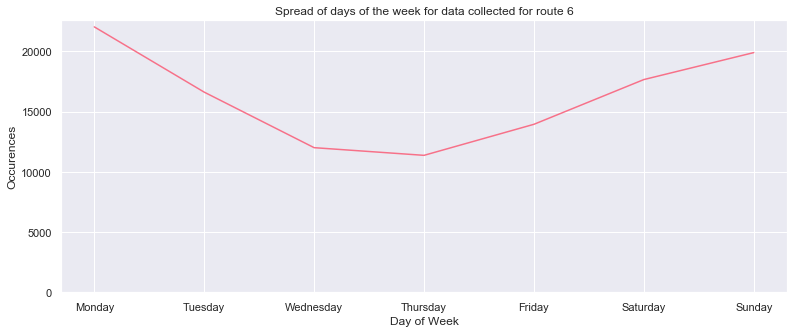
\includegraphics[keepaspectratio, width=15cm]{Images/exploration-spread-dayofweek-6.png}
    \caption{Number of buses during the week for route 6}
    \label{fig:spread-of-buses-over-week-6}
\end{center}
\end{figure}

For each route, two bus stops were chosen and the travel times of the bus were calculated. The z-score (Equation \ref{eqn:z-score}) was calculated for each journey time and used to measure whether a journey time was an outlier or not. A z-score of larger than 3 or smaller than -3 indicates an outlier \cite{significance-of-eda}. 

\begin{equation}
    z = \frac{x_i - \mu}{\sigma}
    \label{eqn:z-score}
\end{equation}

\noindent Where $x_i$ is a journey time, $\mu$ is the mean and $\sigma$ is the standard deviation. The number of occurrences of a travel time was plotted against the actual travel time, marking the outliers in a different colour. An example of this is seen in Figure \ref{fig:outlier-occurences-52} and Figure \ref{fig:outlier-occurences-9}. Figure \ref{fig:outlier-occurences-52} shows the travel times of bus route 52 between 'All Souls Avenue' and 'Nottinghill Gate Station', whilst Figure \ref{fig:outlier-occurences-9} shows the travel times of bus route 9 between 'North End Road' and 'Phillimore Gardens'. In both figures the outliers are marked in green.

\begin{figure}[H]
\begin{center}
    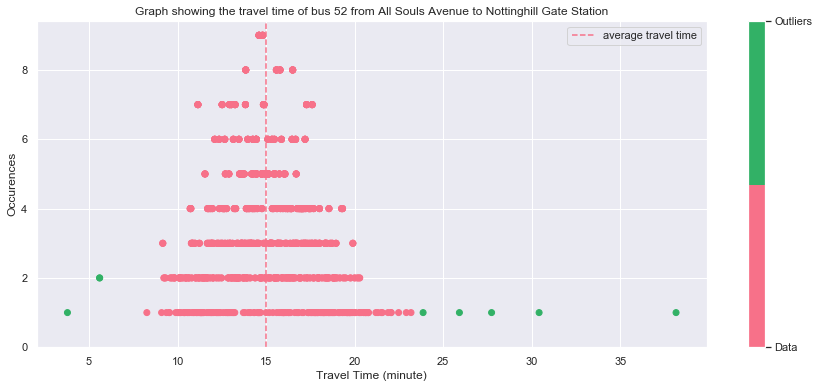
\includegraphics[keepaspectratio, width=15cm]{Images/outliers-52.png}
    \caption{Route 52 travel time and outliers}
    \label{fig:outlier-occurences-52}
\end{center}
\end{figure}

\begin{figure}[H]
\begin{center}
    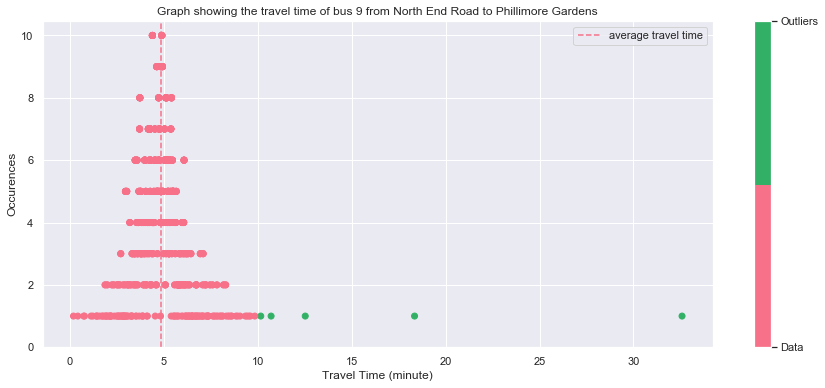
\includegraphics[keepaspectratio, width=15cm]{Images/outliers-9.png}
    \caption{Route 9 travel time and outliers}
    \label{fig:outlier-occurences-9}
\end{center}
\end{figure}

The outliers that have been identified for each route were then removed from the dataset so that the models developed using the data would not be affected by them. \\

The variance and standard deviation were also calculated. For the journey times for buses on route 52 between 'All Souls Avenue' and 'Nottinghill Gate Station', the standard deviation was 2.761 (3sf) and the variance was 7.624 (3sf). For the journey times for buses on route 9 between 'North End Road' and 'Phillimore Gardens', the standard deviation was 1.759 (3sf) and the variance was 3.095 (3sf). 'All Souls Avenue' and 'Nottinghill Gate Station' are 16 stops apart whilst 'North End Road' and 'Phillimore Gardens' are 5 stops apart. Therefore, it was hypothesised that the standard deviation and variance for journey times are lower for stops that are closer to each other. In order to confirm this, 'Aldwych / Somerset House' was chosen as the start stop and the variance and standard deviation of the journey times between the start stop and stops further away on route 6 were calculated. The results for between two stop away to twenty stops away can be seen in Figure \ref{fig:variance-sd-6}.

\begin{figure}[H]
\begin{center}
    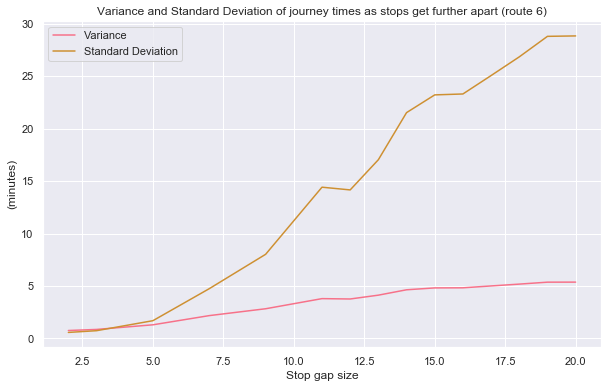
\includegraphics[keepaspectratio, width=13cm]{Images/expolration-variance-sd.png}
    \caption{Route 6 Variance and Standard Deviation}
    \label{fig:variance-sd-6}
\end{center}
\end{figure}

Based on the results as seen in Figure \ref{fig:variance-sd-6}, it is possible to conclude that there is indeed an upward trend in the variance and standard deviation for stops that are further apart. Therefore, predictions made for bus stops that are closer together are likely to be more accurate. 

\subsubsection{Effect of time of day and day of week}

To see the effect of time of day on bus journey times, the times of day were split into eight sections: 00-03, 03-06, 06-09, 09-12, 12-15, 15-18, 18-21, 21-00. For each route two bus stops were chosen and the travel times of the bus were calculated and plotted, as in Figure \ref{fig:time-of-day-69} and Figure \ref{fig:time-of-day-52}. Figure \ref{fig:time-of-day-69} shows the travel times of buses from Florence Road to Star Lane on route 69, which are five stops apart. Figure \ref{fig:time-of-day-52} shows the travel times of buses from All Souls Avenue to Notting Hill Gate Station on route 52, which are 16 stops apart. The Figures also have the average journey time across all hours of the day plotted as a black dotted line. 

\begin{figure}[H]
\begin{center}
    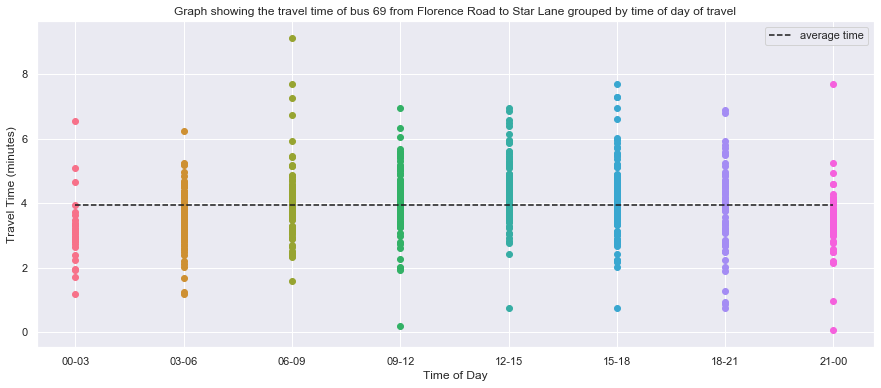
\includegraphics[keepaspectratio, width=15cm]{Images/journey-grouped-by-time-of-day-69.png}
    \caption{Route 69 travel time grouped by time of day}
    \label{fig:time-of-day-69}
\end{center}
\end{figure}

\begin{figure}[H]
\begin{center}
    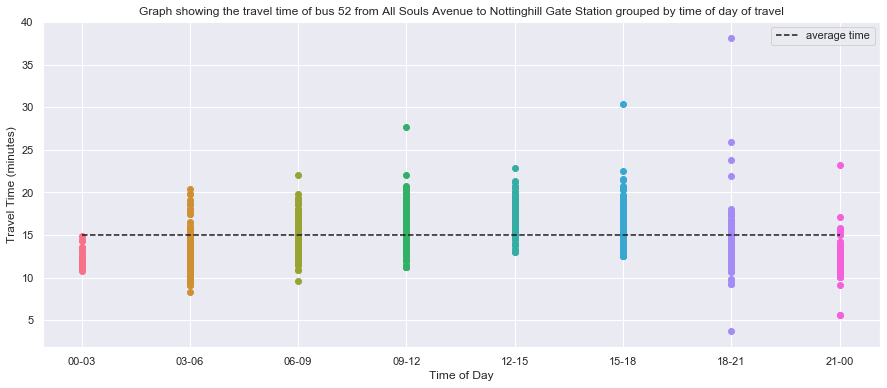
\includegraphics[keepaspectratio, width=15cm]{Images/journey-grouped-by-time-of-day-52.png}
    \caption{Route 52 travel time grouped by time of day}
    \label{fig:time-of-day-52}
\end{center}
\end{figure}

To see the effect of the day of week on bus journey times, the days of the week were split into weekdays versus weekends. As above, for each route two bus stops were chosen and the travel times calculated and plotted. An example can be seen in Figure \ref{fig:day-of-week6}, which shows the travel times for a bus on route 6 from Marble Arch to Church Street Market. It can be seen that there does not seem to be a marked difference between weekday versus weekend journey times. 

\begin{figure}[H]
\begin{center}
    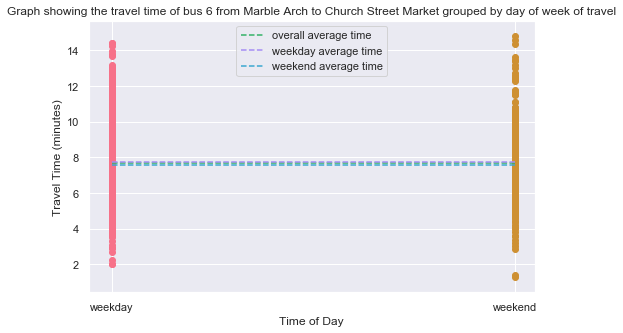
\includegraphics[keepaspectratio, width=12cm]{Images/exploration-dayofweek6.png}
    \caption{Route 6 travel time grouped by day of week}
    \label{fig:day-of-week6}
\end{center}
\end{figure}

\subsubsection{Effect of COVID-19 lockdown}

To see the effect of the lockdown in London on bus journey times, the journeys were split into journeys that occurred during lockdown and journeys that occurred prior or post lockdown. In this case, lockdown was considered to have begun from 24th March 2020 up to 31st May 2020, when the government began easing restrictions on travel \cite{lockdown-easing}. As before, pairs of bus stops were chosen and the travel times calculated and plotted. Figure \ref{fig:lockdown6} shows an example of travel times for a bus on route 6 from Marble Arch to Church Street Market. Due to the reduced number of vehicles on the road and the reduced number of passengers, it was hypothesised that journey times during the lockdown period would be less than journey times outside of this period. This is confirmed by the Figure \ref{fig:lockdown6}. 

\begin{figure}[H]
\begin{center}
    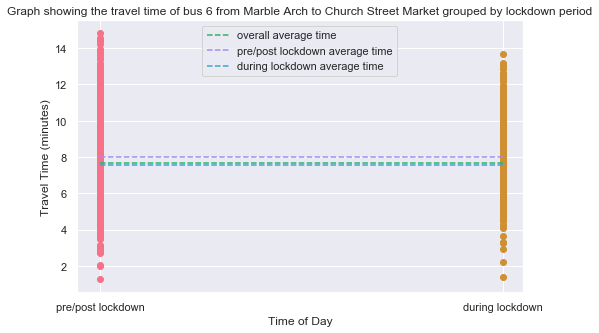
\includegraphics[keepaspectratio, width=12cm]{Images/exploration-lockdown6.png}
    \caption{Route 6 travel time grouped by lockdown period}
    \label{fig:lockdown6}
\end{center}
\end{figure}

\subsubsection{Conclusions}

It was hypothesised that there would be a morning and afternoon peak where journey times would be longer. This is not so obvious in Figure \ref{fig:time-of-day-52} and Figure \ref{fig:time-of-day-69}, however, it can be seen that in the early morning and late night hours (approximately 2100 - 0300), the journey times are generally shorter than other times of day. Therefore, time of day was decided to be chosen to explore as a factor affecting bus journey times. \\

It was also hypothesised that although overall journey times would not be vastly different between weekdays and weekends, it was likely that the morning peak or afternoon peak would be at different times for the weekend compared to weekdays. For this reason, day of week was still chosen to be explored further as a factor affecting bus journey times. \\

However, whether a journey was made during lockdown or not was not chosen as a factor to be explored further. This is because, data from June 2020 onwards will no longer count as being in the lockdown period. Therefore, predictions using recent data will have no recent data that qualify as during lockdown.

\subsubsection{Technology Choices}

As with the previous section, Python was again chosen as the language to implement the data exploration code in. Furthermore, Jupyter Notebook was chosen to write and run the code in.  

\subsection{Historical Models}
\label{section:historical-model-design}

The historical model is a combination of the mean and naive forecasting methods; it takes the weighted average of the journey times looking back at either a different number of buses or different amounts of time. \\

The hypothesis is that the journey time of a bus is dependent on the journey times of recent buses that also completed this journey. Therefore, to explore what `recent' means in this case, the algorithm looks back at 1) different amounts of time and 2) different numbers of buses. The point of looking only at recent data is to ensure that the prediction is able to react to new changes. For example, if there has been an accident on the road, then it would make sense to assume that journeys soon after this accident would take longer. However, if this accident happened far enough into the past, for example an hour ago, it would also be reasonable to assume that this would no longer affect the journey times of vehicles now. \\

If the user gets on bus route X at stop A and requests the estimated arrival time at stop B, the algorithm by which this time is predicted is shown in Figure \ref{fig:historical-flow}: 

\begin{figure}[H]
\begin{center}
    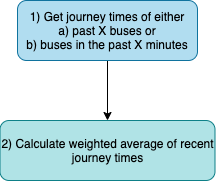
\includegraphics[keepaspectratio, width=6cm]{Images/Historical-Model-overarch.png}
    \caption{Overarching historical model}
    \label{fig:historical-flow}
\end{center}
\end{figure}

\textbf{1) Get recent journey times}: To ensure a wide enough breadth of `recent' journey times to explore, eight submodels are explored.

\begin{enumerate}[label=(\alph*)]

\item Looking back different amounts of time: The historical model looks back at buses from the past 15 minutes, 30 minutes, 60 minutes and 120 minutes. 

\item Looking back different numbers of buses: The historical model looks back at the last 2 buses, 5 buses, 10 buses and 15 buses.

\end{enumerate} 

\textbf{2) Calculate weighted average of recent journey times}: It is necessary to calculate the weighted average of the recent journey times because it is unlikely that the journey time of a bus 100 minutes before the request time will have as much of an effect on the current journey. Using grid search cross validation, the weights are tuned such that they give the optimal predictions. Let $t$ be the amount of time that a bus arrived at stop B before the request time. Let $n$ be the nth most recent bus to arrive at stop B before the request time. For example, $t = 10$ implies that the bus arrived at stop B 10 minutes before the request time and $n=1$ implies that bus was the most recent to arrive at stop B before the request time. The final weightings are as follows:

\begin{itemize}
    \item Weights for the past 15 minutes: $0 < t \leq 10: 0.65, 10 < t \leq 15: 0.35$
    \item Weights for the past 30 minutes: $0 < t \leq 10: 0.65, 10 < t \leq 20: 0.3, 20 < t \leq 30: 0.05$ 
    \item Weights for the past 60 minutes: $0 < t \leq 10: 0.65, 10 < t \leq 20: 0.2, 20 < t \leq 40: 0.1, 40 < t \leq 60: 0.05$ 
    \item Weights for the past 120 minutes:$0 < t \leq 10: 0.65, 10 < t \leq 20: 0.18, 20 < t \leq 40: 0.1, 40 < t \leq 80: 0.05, 80 < t \leq 120: 0.02$ 
    \item Weights for the past 2 buses: $0 < n \leq 2: 1$
    \item Weights for the past 5 buses: $0 < n \leq 2: 0.55, 2 < n \leq 5: 0.45$
    \item Weights for the past 10 buses: $0 < n \leq 1: 0.55, 2 < n \leq 5: 0.35, 5 < n \leq 10: 0.1$
    \item Weights for the past 15 buses: $0 < n \leq 1: 0.45, 2 < n \leq 5: 0.3, 5 < n \leq 10: 0.2, 10 < n \leq 15: 0.05$
\end{itemize}

\subsubsection{Evaluating the model}

The model was evaluated by choosing random pairs of stops and routes and then making requests at thirty minute intervals from 2020/05/25 02:00:00 to 2020/06/08 23:59:59. The root mean squared error (RMSE) and the mean absolute absolute errors (MAE) were calculated and compared against each other. \\

Initially, the eight sub-models were tested on pairs of stops that were five stops apart. Then, the best two of the sub-models were chosen by averaging their RMSE and MAE scores. These were run again using pairs of stops that were further apart to see how well the models generalised to stops that were further apart. As described in Section \ref{section:data-exploration}, the variance in the journey times of the stops increase as the gap between the stops increase. Therefore, the models perform best on stops that are closer together. So, the best overall model is the one that still maintains a good MAE and RMSE for larger gaps.

\subsubsection{Technology Choices}

Python was chosen as the language to develop the models. This is due to the large amount of support for statistical modelling and because I have experience using Python in my Intro Data Science module.

\subsection{Regression + Interpolation Models}

The regression and interpolation model is a two part model that combines two models together to make a prediction. The first model is a regression model and the second model is one of three sub-models: weighted average model, linear regression model and natural cubic spline model. The two sub-models combined form a linear interpolation model. \\

The hypothesis is that the journey time of a bus relies on both `global' conditions and `local' conditions. `Global' conditions in this case refers to factors such as the time of day or the day of the week that have a constant effect throughout history. `Local' conditions on the other hand refers to more recent journey data that could indicate an increase or decrease in journey time. For example, it is assumed that the general trend in travel conditions is more or less the same every weekend - this is a `global' condition. However, if on a particular weekend there is a car crash in the morning that causes journey times to increase, then for this particular weekend, the expected journey time would not be the same as with other weekends - this is a `local' condition. \\ 

This is why a two part model was chosen; so that the first part, the regression model, could calculate the `global' prediction, and then the second part could calculate the `local' prediction. A linear interpolation of the two predictions is then used to calculate the overall prediction of a journey time. \\

Before being able to choose the `global' conditions, it is necessary to explore the different possible features to see if they are correlated to each other or not. If the factors are dependent upon one another, then they cannot be used as separate covariates. 

If the user gets on bus route X at stop A and requests the estimated arrival time at stop B, the algorithm by which this time is predicted is shown in Figure \ref{fig:overarch-combined-model}. \\

\begin{figure}[H]
\begin{center}
    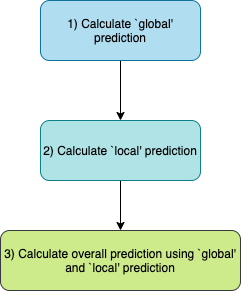
\includegraphics[keepaspectratio, width=6cm]{Images/Regression-Model-overarch.png}
    \caption{Overarching combined model}
    \label{fig:overarch-combined-model}
\end{center}
\end{figure}

1) \textbf{Calculate `global' prediction}: The first part of the model, which is the regression model, predicts the journey time of a bus from stop A to stop B based on the `global' conditions. The chosen factors are the gap size between the stops, the time of day and the day of week. Equation \ref{eq:part1-regression} shows the linear regression model used for the prediction.

\begin{equation}
\label{eq:part1-regression}
    y_{pred1} = b_0 + b_1x_1 + b_2x_2 + b_3x_3 + ... + b_{26}x_{26}
\end{equation}

where 
\begin{itemize}
    \item $x_1$ is the number of stops apart stop A and stop B are (gap size).
    \item $x_2$ is a binary value \{0, 1\} representing the day of week, where 0 is weekday and 1 is weekend
    \item $x_3 ... x_{26}$ is the one hot encoding of the time of day where $x_i$ represents the (i-3)th hour of the day, for i = [3,26]. e.g. $x_3$ represents the 0th hour of the day i.e. between 00:00 and 00:59
    \item $y_{pred1}$ is the predicted journey time of a bus from stop A to stop B based on `global' conditions.
\end{itemize}

Figure \ref{fig:part1-regression-input} is an example of the data that is used to train the regression model. The `Journey Time (s)' column is the $y$ truth values to compare against the $y_{pred1}$ predicted values. The remaining columns are the $x$ training values fed into the model.

\begin{figure}[H]
\begin{center}
    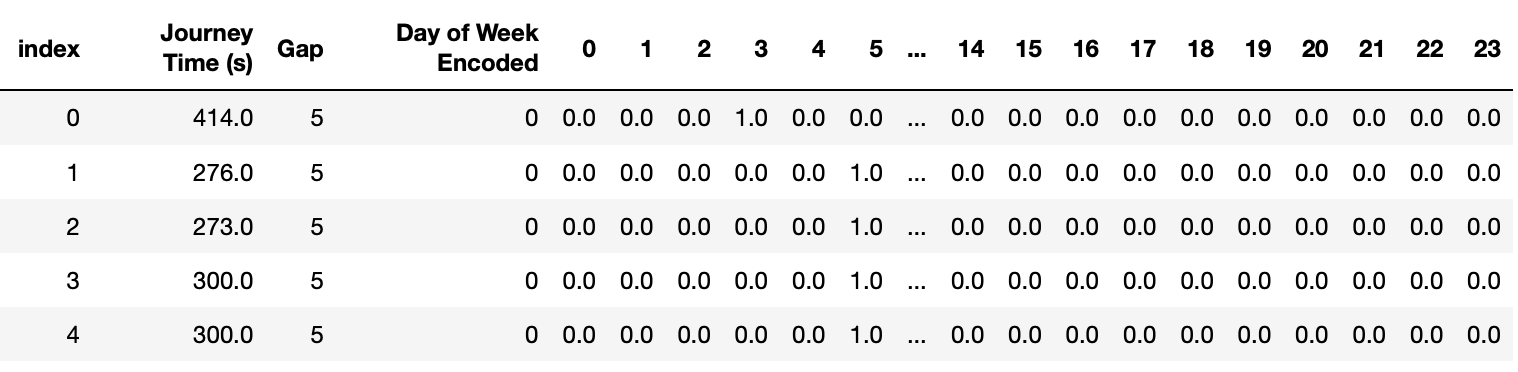
\includegraphics[keepaspectratio, width=15cm]{Images/regression-input.png}
    \caption{Part 1 Regression input example}
    \label{fig:part1-regression-input}
\end{center}
\end{figure}

In order to evaluate the quality of the regression model, requests are made from 20/04/2020 01:00:00 to 08/06/2020 23:59:59 at thirty minute intervals for a number of different pairs of stops of varying routes and gap sizes. The root mean squared error (RMSE), R2-score and mean absolute error (MAE) were then calculated and the results are shown below:  

\begin{itemize}
    \item RMSE: 343.09 seconds (5sf)
    \item R2-score: 0.86865 (5sf)
    \item MAE: 224.58 seconds (5sf)
\end{itemize}

Since an R2-score of 1 means a perfect prediction and the R2-score is bounded between 0 and 1, a score of 0.85749 indicates that the model gives a fairly good prediction of the journey time. However, the MAE and RMSE score indicate that the predictions can be around 4 and 6 minutes off respectively, which in reality is not very good at all. This supports the hypothesis that recent data, i.e. the `local' conditions, need to also be taken into account as looking at these `global' factors alone does not provide an accurate enough prediction. \\

The model is pre-trained and therefore, for this step, the algorithm need only gather the required features and put them into Equation \ref{eq:part1-regression} to get $y_{pred1}$. The intercept and coefficient have already been pre-computed and are as follows:

\begin{itemize}
    \item Coefficients: [[ 7.78320354e+02 -2.15578663e+01  5.73810236e+12  6.16413662e+12
   6.90322104e+12  9.84142661e+12  1.12486687e+13  1.41533295e+13
   1.78363604e+13  1.87106607e+13  1.92728119e+13  2.02578876e+13
   2.12199016e+13  2.17152238e+13  2.01181975e+13  1.96601961e+13
   2.00780471e+13  2.12757351e+13  2.06500324e+13  1.84661903e+13
   1.53716651e+13  1.15428232e+13  1.10275325e+13  9.32177162e+12
   1.05914818e+13  6.93639804e+12]]
   \item Intercept: [1078.31645828]
\end{itemize}

This calculated $y_{pred1}$ is stored for further use in step 3). \\

2) \textbf{Calculate `local' prediction}: The second part of the model predicts the journey time of a bus from stop A to stop B based on the `local' conditions, which in this case is the last 10 buses to travel from stop A to stop B. It was decided to look back 10 buses because based on the historical models as described in Section \ref{section:historical-model-design}, the model that looked back 10 buses performed the best. There are three different sub-models that were used: \\

\begin{itemize}
    \item \textbf{Weighted Average}
    \begin{equation}
        y_{pred2} = weighted\ average\ of\ last\ 10\ journeys
    \end{equation}
    where the weights are the same as in Section \ref{section:historical-model-design}: up to 2 buses = 0.55, between 2 to 5 buses = 0.35, between 5 to 10 buses = 0.1. This makes this sub-model essentially the same model as the historical average model. A weighted average model is good for cancelling out rivalling effects or when the data is noisy. However, it does not indicate trends in the data. For example, as seen in Figure \ref{fig:weighted-avg-regression} if the last 10 journeys are decreasing in journey time, it might be assumed that at the current request time, the journey time would be even less, following the downward trend. However, the weighted average model is unable to provide such a prediction.
    
    \begin{figure}[H]
    \begin{center}
        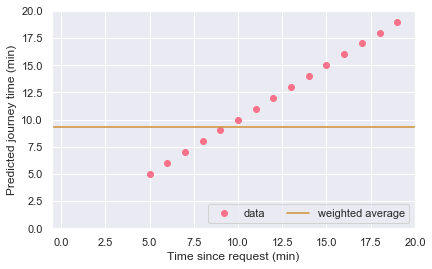
\includegraphics[keepaspectratio, width=10cm]{Images/regression-weightedavg.png}
        \caption{Unable to capture trend}
        \label{fig:weighted-avg-regression}
    \end{center}
    \end{figure}
    
    \item \textbf{Linear Regression}
    \begin{equation}
        y_{pred2} = linear\ regression\ based\ on\ last\ 10\ journeys
    \end{equation}
    
    If the y axis is the journey time and the x axis is the time since the request, then $y_{pred2}$ is the intercept with the y axis. It is undesirable to use a regression model with degree larger than 1 because at the extremes the values become very large or very small. Thus, the intercept, would also be very large or very small and not close enough to the desired predicted value. This is demonstrated in Figure \ref{fig:extreme-bestfit}, which shows the journey times of the last 10 journeys alongside the regression models. It could be inferred from the last 10 journey times that the bus journey time at the request time (i.e. at 0 on the x axis) would be somewhere in between 5 and 7 minutes. This is captured best with the model with degree = 1.
    
    \begin{figure}[H]
    \begin{center}
        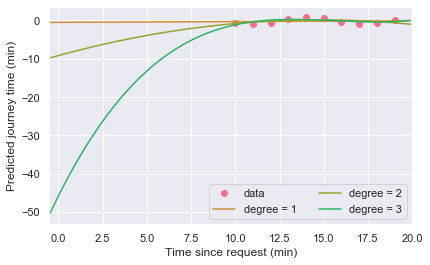
\includegraphics[keepaspectratio, width=10cm]{Images/regression-lineofbestfit.png}
        \caption{Intercept becomes more extreme}
        \label{fig:extreme-bestfit}
    \end{center}
    \end{figure}
    
    \item \textbf{Cubic Spline Interpolation}
    \begin{equation}
        y_{pred2} = fit\ a\ cubic\ spline\ to\ the\ last\ 10\ journeys
    \end{equation}
    
    Similarly to the linear regression case, the y axis is the journey time, the x axis is the time since the request and the intercept is $y_{pred2}$. Cubic splines with three different types of boundary conditions were used: `not-a-knot', `clamped' and `natural'. `not-a-knot' indicates that the first and second segment at a curve end are the same. `clamped' indicates that the first derivative at the curves' ends are zero. `natural' indicates that the second derivatives at the curves' ends are zero. Figure \ref{fig:three-bounary-conditions} demonstrates that the 'not-a-knot' and 'clamped' conditions provide more extreme intercept values than the 'natural' condition.
    
    \begin{figure}[H]
    \begin{center}
        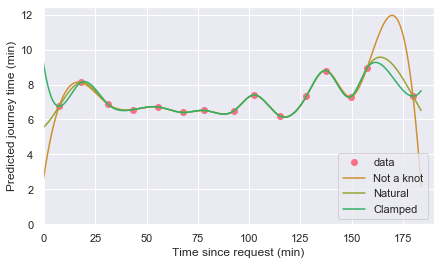
\includegraphics[keepaspectratio, width=10cm]{Images/regression-cubicspline.png}
        \caption{Three Boundary Conditions}
        \label{fig:three-bounary-conditions}
    \end{center}
    \end{figure}

\end{itemize}

All three `local' models were used in the training process, but only the best performing one will be used in the mobile app. The input to all three models is simply the journey times of the most recent fifteen journeys from stop A to stop B and how long ago the bus arrived at stop B compared to the request time. Therefore, $y\_{pred2}$ can be calculated in such a manner and is stored for further use in step 3).\\

\textbf{3) Calculate overall prediction using `global' and `local' prediction}: The last part of the model combines $y_{pred1}$ with $y_{pred2}$ to form Equation \ref{eq:regression-overall} for the overall prediction. This is essentially a linear interpolation model:

\begin{equation}
\label{eq:regression-overall}
    y_{pred} = \alpha y_{pred1} + (1 - \alpha)y_{pred2}
\end{equation}

where 
\begin{itemize}
    \item $y_{pred}$ is the overall journey time prediction for a bus travelling from stop A to stop B at the request time.
    \item $\alpha$ is some coefficient that we are looking to find such that it minimises the validation root mean squared error (RMSE) and mean absolute error (MAE). 
\end{itemize}

Parameter tuning on $\alpha$ is performed on $y_{pred1}$ and all five $y_{pred2}$ values, with $\alpha$ varying from zero to one. Based on the hypothesis, it is assumed that the optimal value of $\alpha$ is achieved around the region of 0.5 because this would indicate that an equal contribution from the `global' and `local' models are required in order to get the overall predicted value.

\subsubsection{Model Evaluation}

The overall model was evaluated in the same way part one of the model is evaluated: requests are made from 25/05/2020 02:00:00 to 08/06/20 23:59:59 at thirty minute intervals for a number of different pairs of stops of varying routes and gap sizes. The root mean squared errors (RMSE) and mean absolute errors (MAE) were calculated for the five possible models (due to the five possibilities for part two of the model) and compared against each other. \\

It should be noted that looking back at the last 10 buses was the best model out of all the historical average models and one of the `local' models is a weighted average historical model. Therefore, it is likely that the overall model that performs the best is the one that has the weighted average model as the `local' model. Furthermore, if the `local' models instead had chosen to look back at e.g. the last 5 buses or buses in the past two hours, it is possible that a different `local' model would lead to the best overall model.

\subsubsection{Technology Choices}

As with the Historical Models, Python was the language used to develop the models. This was due to the large amount of built in help for regression and interpolation that comes with the \texttt{sklearn} library. 

\subsection{Phone App}

\subsubsection{Front End}

\subsubsection{Back End}

\clearpage